\documentclass[11pt]{beamer}
\setbeamertemplate{navigation symbols}{}
 \setbeamercovered{transparent}
\usepackage{listings}
%\usetheme{Copenhagen}
\usetheme{Singapore}
%\usetheme{Madrid}
%\usetheme{Hannover}
%\usetheme{boxes}
%\usetheme{Boadilla}
\usefonttheme[onlymath]{serif}
\usecolortheme{beaver}
\usepackage{textpos}
\usepackage{fancyvrb}
\usepackage{xcolor}
\usepackage{multicol}
\usepackage{lipsum}
\parskip 1ex

\newcommand\FontAcolumn{\fontsize{6}{7.2}\selectfont}
\newcommand\FontBcolumn{\fontsize{8}{7.2}\selectfont}
\newcommand\FontCcolumn{\fontsize{10}{7.2}\selectfont}
\newcommand\FontDcolumn{\fontsize{11}{7.2}\selectfont}

\definecolor{gray97}{gray}{.97}
\definecolor{gray75}{gray}{.75}
\definecolor{gray75}{gray}{.45}

\lstdefinestyle{Fortran}{language=[90]Fortran}

\newcommand\FortranStyle
{
\lstset{
frame=Ltb,
framerule=0pt,
columns=fullflexible,
aboveskip=0.5cm,
framextopmargin=3pt,
framexbottommargin=3pt,
framexleftmargin=0.4cm,
framesep=0pt,
rulesep=.4pt,
backgroundcolor=\color{gray97},
rulesepcolor=\color{black},
stringstyle=\ttfamily,
showstringspaces=false,
basicstyle=\ttfamily,
commentstyle=\color{green},
keywordstyle=\color{red},
numbers=left,
numbersep=15pt,
numberstyle=\tiny,
numberfirstline=false,
breaklines=true,
 tabsize=2,
 extendedchars=true,
keepspaces,
}
}

\newcommand\FortranStyleA
{
\lstset{
frame=Ltb,
framerule=0pt,
columns=fullflexible,
aboveskip=0.5cm,
framextopmargin=3pt,
framexbottommargin=3pt,
framexleftmargin=0.4cm,
framesep=0pt,
rulesep=.4pt,
backgroundcolor=\color{gray97},
rulesepcolor=\color{black},
stringstyle=\ttfamily,
showstringspaces=false,
basicstyle=\ttfamily,
commentstyle=\color{green},
keywordstyle=\color{red},
numbersep=15pt,
numberstyle=\tiny,
numberfirstline=false,
breaklines=true,
 tabsize=2,
 extendedchars=true,
keepspaces,
}
}

\newcommand\tab[1][1cm]{\hspace*{#1}}
\newcommand{\light}[1]{\textcolor{lightgray}{#1}}
    
\def\signed #1{{\leavevmode\unskip\nobreak\hfil\penalty50\hskip2em
  \hbox{}\nobreak\hfil(#1)%
  \parfillskip=0pt \finalhyphendemerits=0 \endgraf}}

\newsavebox\mybox
\newenvironment{aquote}[1]
  {\savebox\mybox{#1}\begin{quote}}
  {\signed{\usebox\mybox}\end{quote}}
  
% items enclosed in square brackets are optional; explanation below
\title{Array Concepts}
\author{Carlos Cruz}
\institute{
  NASA GSFC Code 606 (ASTG)\\
  Greenbelt, Maryland 20771\\[1ex]
  \texttt{carlos.a.cruz@nasa.gov}
}
\date{October 24, 2018}

\begin{document}

% --- Title page ---
\begin{frame}[plain]
  \titlepage
\end{frame}

\logo{%
  
\includegraphics[width=1cm,height=1cm,keepaspectratio]{../../shared/nasa-ball.png}%
  \hspace{\dimexpr\paperwidth-2cm-5pt}%
  
\includegraphics[width=1cm,height=1cm,keepaspectratio]{../../shared/ssai-logo.png}%
}

% --- Slide

\begin{frame}{Agenda}

\textcolor{red}{Array Concepts}
    \begin{itemize}
        \item Terminology
        \item Declarations
        \item Syntax
        \item Expressions
        \item Intrinsic functions
        \item Allocatable arrays
    \end{itemize}
 
\end{frame}


% --- Slide

\begin{frame}[fragile]
\frametitle{Array Declarations}

\footnotesize{
 \begin{itemize}
\item Default lower bound is 1
\item Bounds can begin and end anywhere
\item Arrays can be zero-sized
\item Up to 7 dimensions
\end{itemize}
  \FortranStyle
\begin{lstlisting}[style=Fortran]
    real, dimension(15)       :: A ! static arrays
    real, dimension(-4:0,0:2) :: B
    real F(360,180) 
    integer, dimension(20)    :: N
    
    integer, parameter :: UB = 5 ! Literals and constants can
    real, dimension(0:UB-1)   :: Y ! be used in array 
    real, dimension(1+UB*UB,10) :: Z ! declarations
\end{lstlisting}
 }
\end{frame}

% --- Slide

\begin{frame}[fragile]
\frametitle{Array Terminology}

\begin{columns}
  \begin{column}{0.5\textwidth}
  \FortranStyle
    \FontBcolumn
\begin{lstlisting}[style=Fortran]
real, dimension(15)       :: A
real, dimension(-4:0,0:2) :: B
real C(5,3), D(0:4,0:2) 
\end{lstlisting}
A:\\
\quad rank=1, size=15, shape=15\\
B:\\
\quad rank=2, size=15, shape=5x3\\
C:\\
\quad rank=2, size=15, shape=5x3\\
D:\\
\quad rank=2, size=15, shape=5x3\\
\vspace{5mm}
B,C,D are conformable\\

\end{column}

  \begin{column}{0.4\textwidth}
  \FontBcolumn
 \begin{itemize}
 \item \emph{rank} : number of dimensions
 \item \emph{bounds} : upper and  lower limits of indices
\item \emph{extent} : number of elements in dimensions
\item \emph{size} : total number of elements
\item \emph{shape} : rank and extents
\item \emph{conformable} : same shape, B and C and D
 \end{itemize}
 \end{column}
\end{columns}
\bigskip
 
\end{frame}

% --- Slide

\begin{frame}{Array visualization}


\begin{figure}[t]
\centering
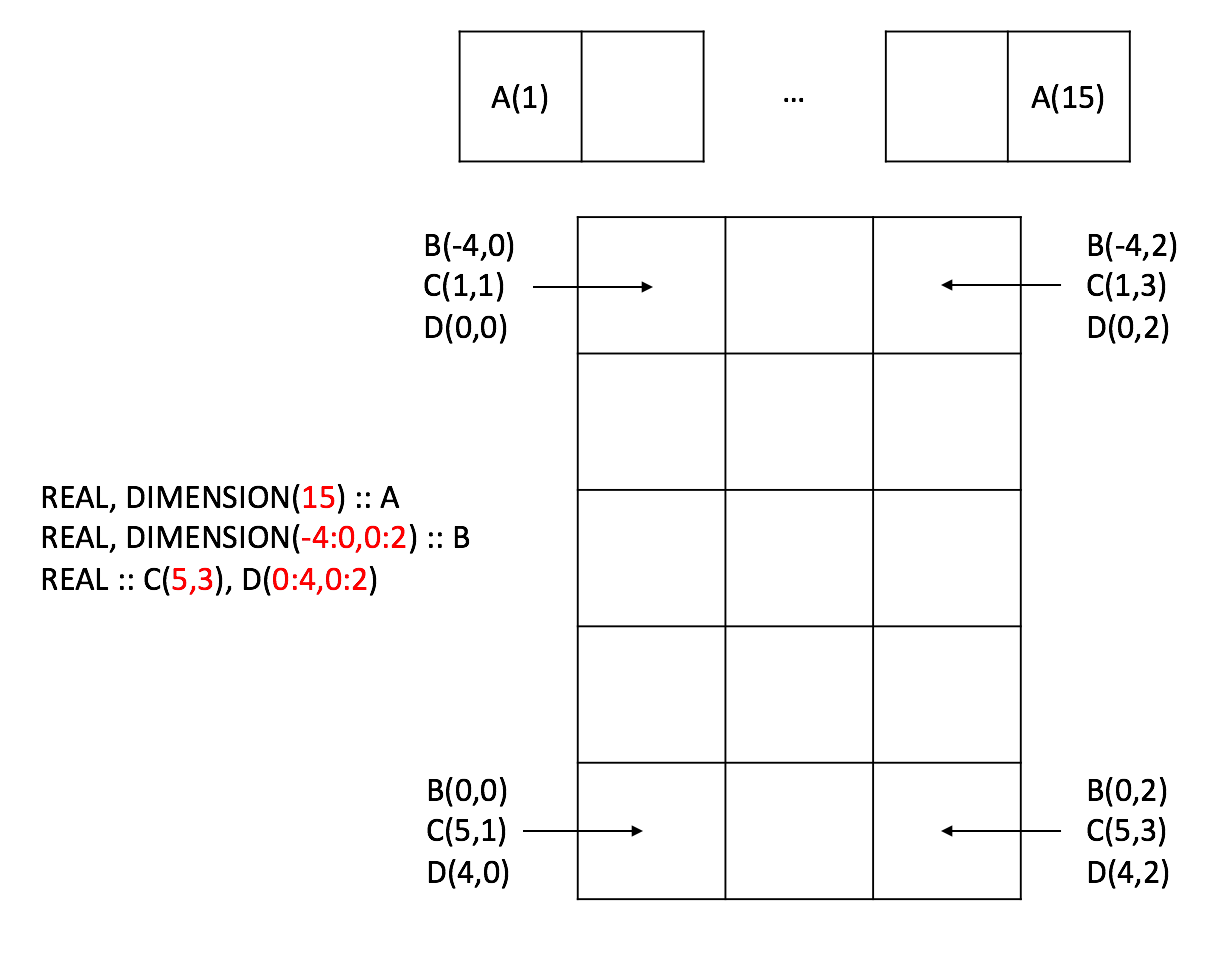
\includegraphics[scale=.4]{../../shared/array_vis2.png}
\end{figure}
  
% Data layout is critical for correctly passing arrays between programs written in different programming languages. It is also important for performance when traversing an array because modern CPUs process sequential data more efficiently than nonsequential data. This is primarily due to CPU caching. In addition, contiguous access makes it possible to use SIMD instructions that operate on vectors of data. In some media such as tape or NAND flash memory, accessing sequentially is orders of magnitude faster than nonsequential access

\end{frame}


% --- Slide

\begin{frame}[fragile]
\frametitle{Array Syntax}

Using the earlier declarations, references can be made to:

\begin{itemize}
\item whole arrays (conformable)\\
%\begin{itemize}
\quad \textcolor{blue}{A = 0} $\leftarrow$ sets whole array A to zero \\
\quad \textcolor{blue}{B = C + 1} $\leftarrow$ adds one to all elements, of C \\
\quad \quad \quad and then assigns each element to the corresponding \\
\quad \quad \quad element of B \\
%\end{itemize}

\item elements \\
%\begin{itemize}
\quad \textcolor{blue}{A(1) = 0.0} $\leftarrow$ sets one element to zero \\
\quad \textcolor{blue}{B = A(3) + C(5,1)} $\leftarrow$ sets whole array B to the sum of \\
\quad \quad \quad two elements\\
%\end{itemize}

\item array sections \\
%\begin{itemize}
\quad \textcolor{blue}{A(2:6) = 0} $\leftarrow$ sets section of A to zero \\
\quad \textcolor{blue}{B(-1:0,1:2) = C(1:2,2:3) + 1} $\leftarrow$  adds one to the subsection \\
\quad \quad \quad of C and assigns it to the subsection of B \\
% \end{itemize}
 \end{itemize}
%\bigskip
 
\end{frame}

% --- Slide

\begin{frame}[fragile]
\frametitle{Array Expressions}

Arrays can be treated like a single variable in that:
\begin{itemize}
\item can use intrinsic operators between conformable arrays (or sections)
\begin{itemize}
\item \textcolor{blue}{B = C * D - B**2}
 \end{itemize}

\item elemental intrinsic functions can be used
\begin{itemize}
\item \textcolor{blue}{B = sin(C) + cos(D)}
 \end{itemize}

 \end{itemize}
\bigskip
 
\end{frame}


% --- Slide

\begin{frame}[fragile]
\frametitle{Array Expressions}

\footnotesize{
An array can be subscripted by a \emph{subscript-triplet} giving rise to a sub-array of the original. The general form is: \\
\quad \quad \emph{(start:end:stride)} \\

the section starts at \emph{start} and ends at or before \emph{end}.\emph{stride}  is the increment by which the locations are selected. \\
\emph{start, end, stride} must all be scalar integer expressions. Thus, these are all valid:
  \FortranStyle
\begin{lstlisting}[style=Fortran]
	A(m:m) = 0     ! m to m, 1 element array
	A(m:n:k) = 0   ! m to n step k
	A(8:3:-1) = 0  ! 8 to 3 backwards
	A(8:3) = 2     ! step 1 => zero size
	A(m::4) = 1    ! default UPB, step 4
	A(::2) = 1.0   ! default LWB and UPB
	A(m**2:n*k/3) = 1.0
\end{lstlisting}
}
\end{frame}


% --- Slide

\begin{frame}[fragile]
\frametitle{Array Inquiry (1)}

\footnotesize{
Consider the declaration:
  \FortranStyle
\begin{lstlisting}[style=Fortran]
real, dimension(-10:10,23,14:28) :: A
\end{lstlisting}
 Then:
\begin{itemize}
\item LBOUND(SOURCE[,DIM]) -- lower bounds of an array (or bound in an optionally specified dimension).
\begin{itemize}
\item LBOUND(A) is (/-10,1,14/) (array).
\item LBOUND(A,1) is -10 (scalar)
 \end{itemize}
 \item UBOUND(SOURCE[,DIM]) -- upper bounds of an array (or bound in an optionally specified dimension).
 \end{itemize}
}

\end{frame}

% --- Slide

\begin{frame}[fragile]
\frametitle{Array Inquiry (2)}
\footnotesize{
 \FortranStyle
\begin{lstlisting}[style=Fortran]
real, dimension(-10:10,23,14:28) :: A
\end{lstlisting}
\begin{itemize}
\item SHAPE(SOURCE) -- shape of an array.
\begin{itemize}
\item SHAPE(A) is (/21,23,15/) (array).
\item SHAPE((/4/)) is (/1/) (array)
 \end{itemize}
 
 \item SIZE(SOURCE[,DIM]) -- total number of array elements (in an optionally specified dimension).
\begin{itemize}
\item SIZE(A,1) is 21.
\item SIZE(A) is 7245
 \end{itemize}
 \end{itemize}
}

\end{frame}

% --- Slide
\begin{frame}[fragile]
\frametitle{Array Constructors}

\footnotesize{
Used to give arrays or sections of arrays specific values. For example,
  \FortranStyle
 \begin{lstlisting}[style=Fortran]
    implicit none
    integer                        :: i
    integer, dimension(10)         :: ints
    character(len=5), dimension(3) :: colors
    real, dimension(4)             :: heights
    heights = (/5.10, 5.6, 4.0, 3.6/)
    colors = (/'RED  ','GREEN','BLUE '/)
    ! note padding so strings are 5 chars
    ints    = (/ 100, (i, i=1,8), 100 /)
\end{lstlisting}
 Then:
\begin{itemize}
\item constructors and array sections must conform.
\item must be 1D.
\item for higher rank arrays use RESHAPE intrinsic
 \end{itemize}
}

\end{frame}

% --- Slide
\begin{frame}[fragile]
\frametitle{Array Constructors in Initialization Statements}

\footnotesize{
Named array constants can be created
\FortranStyle
 \begin{lstlisting}[style=Fortran]
integer, dimension(3), parameter :: &
    unit_vec = (/1,1,1/)
character(len=*), dimension(3),  parameter :: &
    lights =  (/'red  ','blue ','green'/)
real, dimension(3,3), parameter :: &
    unit_matrix = reshape( &  ! using reshape
    (/1,0,0,0,1,0,0,0,1/),(/3,3/))
\end{lstlisting}
 In the second statement all strings must be same length. 
}

\end{frame}

% --- Slide
\begin{frame}[fragile]
\frametitle{RESHAPE}

\footnotesize{
 RESHAPE is a general intrinsic function which delivers an array of a specific shape: 
\begin{lstlisting}[style=Fortran]
RESHAPE(original_shape, new_shape)
 \end{lstlisting}
 e.g.:
  \FortranStyle
\begin{lstlisting}[style=Fortran]
A = RESHAPE((/1,2,3,4/),(/2,2/))
\end{lstlisting}
A is filled in array element order and looks like: 

\begin{Verbatim}
    1    3
    2    4
 \end{Verbatim}
}

\end{frame}

% --- Slide
\begin{frame}[fragile]
\frametitle{DATA}

\footnotesize{
 Use the DATA when other methods are tedious and/or impossible.  
 \begin{lstlisting}[style=Fortran]
DATA variable / list / ...
 \end{lstlisting}
 e.g.:
  \FortranStyle
\begin{lstlisting}[style=Fortran]
INTEGER :: a(4), b(2,2), c(10)
DATA a /4,3,2,1/
DATA a /4*0/ ! * is not multiplication operator!
DATA b(1,:) /0,0/ 
DATA b(2,:) /1,1/
DATA (c(i),i=1,10,2) /5*1/ 
DATA (c(i),i=2,10,2) /5*2/
\end{lstlisting}
}
\end{frame}

% --- Slide
\begin{frame}[fragile]
\frametitle{Allocatable Arrays}

\footnotesize{
Fortran allows arrays to be created on-the-fly; these are known as \emph{allocatable} arrays and use \emph{dynamic heap} storage. Allocatable arrays are
\begin{itemize}
\item declared like explicit-shape arrays but without the extents and with the ALLOCATABLE attribute.
\begin{itemize}
\item integer, dimension(\textcolor{red}{:}), ALLOCATABLE :: ages
\item real, dimension(\textcolor{red}{:},\textcolor{red}{:}), ALLOCATABLE :: speed
 \end{itemize}
 \item given a size in an ALLOCATE statement which assigns an area of memory to the object.
\begin{itemize}
\item ALLOCATE(ages(1:10), STAT=ierr)
\item ALLOCATE(speed(-lwb:upb,-50:0),STAT=ierr)
%The ALLOCATE statement associates storage with an allocatable array:
 \end{itemize}
\item the optional STAT= field reports on the success of the storage request. If the INTEGER variable ierr is zero the request was successful otherwise it failed. 
 \end{itemize}
}

\end{frame}

% --- Slide
\begin{frame}[fragile]
\frametitle{Deallocating Arrays}

\footnotesize{
Heap storage can be reclaimed using the DEALLOCATE statement:
 \begin{lstlisting}[style=Fortran]
DEALLOCATE(ages,STAT=ierr)
 \end{lstlisting}

\begin{itemize}
\item it is an error to deallocate an array without the ALLOCATE attribute or one that has not been previously allocated space.
\item there is an intrinsic function, ALLOCATED, which returns a scalar LOGICAL values reporting on the status of an array. \\
 \begin{lstlisting}[style=Fortran]
if (ALLOCATED(ages)) DEALLOCATE(ages,STAT=ierr)
 \end{lstlisting}

\item the STAT= field is optional but its use is recommended
\item if a procedure containing an allocatable array which does not have the SAVE attribute is exited without the array being DEALLOCATE d then this storage becomes inaccessible
 \end{itemize}
}

\end{frame}

% --- Slide
\begin{frame}[fragile]
\frametitle{Beware of memory leaks}

It is the program that takes responsibility for allocating and deallocating storage to \textbf{static} variables.\\
However, when using dynamic arrays this responsibility falls to the \textbf{programmer}. 

\begin{itemize}
\item Storage allocated to local variables (in say a subroutine or function - more on this later) must be \textbf{deallocated} before the exiting the procedure. 
\begin{itemize}
\item When leaving a procedure all local variables are deleted from memory and the program releases any associated storage for use elsewhere, however any storage allocated through the ALLOCATE statement will remain "in use" even though it has no associated variable name!
 \end{itemize}
\item Storage allocated, but no longer accessible, cannot be released or used elsewhere in the program and is said to be in an "undefined" state This reduction in the total storage available to the program called is a "memory leak".
 \end{itemize}


\end{frame}



% --- Slide
\begin{frame}[fragile]
\frametitle{Masked Array Assignment - Where Statement}

\footnotesize{
This is achieved using WHERE
 \begin{lstlisting}[style=Fortran]
WHERE (I /= 0) A = B/I
 \end{lstlisting}
the LHS of the assignment must be array valued and the mask, (the logical expression,) and the RHS of the assignment must all conform. \\
For example, if 
\[
B = 
 \begin{pmatrix}
  1.0 & 2.0  \\
  3.0 & 4.0  \\
 \end{pmatrix}
 \]
and
\[
I = 
 \begin{pmatrix}
  2 & 0  \\
  0 & 2  \\
 \end{pmatrix}
 \]
then
\[
A = 
 \begin{pmatrix}
  0.5 & -  \\
  - & 2.0  \\
 \end{pmatrix}
 \]
Only the elements, corresponding to the non-zero elements of I, have been assigned to.
}

\end{frame}

% --- Slide
\begin{frame}[fragile]
\frametitle{Where Construct}

\footnotesize{
There is a block form of masked assignment
  \FortranStyle
\begin{lstlisting}[style=Fortran]
 WHERE(A > 0.0)
     B = LOG(A)
     C = SQRT(A)
  ELSEWHERE
     B = 0.0
  ENDWHERE
\end{lstlisting}
\begin{itemize}
\item the mask must conform to the RHS of each assignment; A, B and C must conform.
\item WHERE ... END WHERE is not a control construct and cannot currently be nested. 
\item the STAT= field is optional but its use is recommended
\item the execution sequence is as follows: evaluate the mask, execute the WHERE block (in full) then execute the ELSEWHERE block
\item the separate assignment statements are executed sequentially but the individual elemental assignments within each statement are (conceptually) executed in parallel
 \end{itemize}
}

\end{frame}

% --- Slide
\begin{frame}[fragile]
\frametitle{Vector-valued subscripts}

\footnotesize{
A 1D array can be used to subscript an array in a dimension. Consider
\begin{lstlisting}[style=Fortran]
    integer, dimension(5) :: V = (/1,4,8,12,10/)
    integer, dimension(3) :: W = (/1,2,2/)
 \end{lstlisting}
\begin{itemize}
\item A(V) is A(1), A(4), A(8), A(12), and A(10).
\item the following are valid assignments:
\begin{lstlisting}[style=Fortran]
    A(V) = 3.5
    C(1:3,1) = A(W)
 \end{lstlisting}
\item it would be invalid to assign values to A(W) as A(2) is referred to twice
\item only 1D vector subscripts are allowed, for example
\begin{lstlisting}[style=Fortran]
    A(1) = SUM(C(V,W))
 \end{lstlisting}
 \end{itemize}
}

\end{frame}


% --- Slide

\begin{frame}[fragile]
\frametitle{Conclusion}

Arrays make Fortran a very powerful language, especially for computationally intensive program development.
\scriptsize{
\begin{itemize}
\item Array syntax allows easy (intuitive) initialization
\item Dynamic memory allocation enables customizable sizing of arrays
\item Many array intrinsic functions (most not discussed here)
\end{itemize}
}

\end{frame}


% --- Slide

\begin{frame}[fragile]
\frametitle{Exercise}

We will solve a computational problem that converts temperatures in Fahrenheit to Kelvin\\
\begin{equation}
K = \frac{5}{9}(F - 32) + 273.15
\end{equation}
Using a text editor open the file exercise.F90 and \emph{complete the empty code blocks}. You will:
\begin{itemize}
\item Perform the conversion
\item Print the F and K values
\item Print the log of F (careful!)
 \end{itemize}
Then build the executable and run the code using the provided Makefile.

\end{frame}

\end{document}
